%
%%%%%%%%%%%%%%%%%%%%%%%%%%%%%%%%%%%%%%%%%%%%%%%%%%%%%%%%%%%%%%%%%%%%%%
% Tina Dissertation
% December 2013, modified to Template June 2015
%%%%%%%%%%%%%%%%%%%%%%%%%%%%%%%%%%%%%%%%%%%%%%%%%%%%%%%%%%%%%%%%%%%%%%
% Documentclass Memoir 
% check memman.pdf for help and information
%%%%%%%%%%%%%%%%%%%%%%%%%%%%%%%%%%%%%%%%%%%%%%%%%%%%%%%%%%%%%%%%%%%%%%
\documentclass[openright,12pt,a4paper]{memoir} 
\usepackage{graphicx}
%\usepackage[utf8]{inputenc} % set input encoding to utf8
\usepackage{array} % for tables 
\usepackage{multirow} % for tables 
\usepackage{multicol} % for tables
\usepackage{tabularx} % for tables
\usepackage{booktabs}
\usepackage{cite}
\usepackage{tabularx}
\usepackage[round]{natbib}
\usepackage{threeparttable}
\DisemulatePackage{setspace}
\usepackage{setspace}
\usepackage{longtable}
\usepackage{tabu}
\usepackage{pdflscape}
%\usepackage{caption}
%\usepackage{lmodern}
\usepackage{url} \usepackage[normalem]{ulem}
\useunder{\uline}{\ul}{}



% defines new column type
\newcolumntype{Z}{$>${\raggedright\arraybackslash}X}

% add a little vertical padding to cramped tables
\setlength{\extrarowheight}{2pt}


%%%%%%%%%%%%%%%%%%%%%%%%%%%%%%%%%%%%%%%%%%%%%%%%%%%%%%%%%%%%%%%%%%
%%% Examples of Memoir customization
%%% enable, disable or adjust these as desired

%%% PAGE DIMENSIONS
% a4paper is by default 210mm wide and 279 mm wide

% default document in memoir is twoside (recto-verso) and openright (new chapter begins on recto page)

% size of the text area
  \settrims{0pt}{0pt}
  \settypeblocksize{230mm}{147mm}{*}
  \setlength{\spinemargin}{27mm}
  \setlength{\foremargin}{36mm}
%\setulmargins{35mm}{45mm}{*}
%\setlength{\marginparwidth}{0mm}
%\setlength{\marginparsep}{0mm}
%\setlength{\textwidth}{140mm}
%\settrimmedsize{0.9\stockheight}{0.9\stockwidth}{*}
%\setlength{\trimtop}{0pt}
%\setlength{\trimedge}{0pt}
%\addtolength{\trimedge}{-\paperwidth}
%\settypeblocksize{*}{\lxvchars}{1.618} % we want to the text block to have golden proportionals
  \setulmargins{*}{*}{1.618} % 50pt upper margins
%\setlrmargins{*}{*}{1.3}
%  \setlrmargins{*}{*}{1} % golden ratio again for left/right margins
  \setheaderspaces{*}{*}{1.618}
  \checkandfixthelayout % to make sure that the layout parameters make sense

%\addtolength{\textwidth}{0cm}
%\addtolength{\textheight}{1.5cm}
%\addtolength{\textwidth}{-2cm}
%\addtolength{\textheight}{+0.5cm}

%%% \maketitle CUSTOMISATION
% For more than trivial changes, you may as well do it yourself in a titlepage environment
%\pretitle{\begin{center}\sffamily\Huge\MakeUppercase}
%\posttitle{\par\end{center}\vskip 0.5em}

%%% ToC (table of contents) APPEARANCE
  \maxtocdepth{subsection} % include subsections
%\renewcommand{\cftchapterpagefont}{}
%\renewcommand{\cftchapterfont}{}     % no bold!

%%% HEADERS \& FOOTERS
  \pagestyle{headings} % try also: empty , plain , headings , ruled , Ruled , companion

%%% CHAPTERS
  \chapterstyle{southall} % try also: default , section , hangnum , companion , article, demo

  \renewcommand{\chaptitlefont}{\LARGE\sffamily\raggedright} % set sans serif chapter title font
  \renewcommand{\chapnumfont}{\LARGE\sffamily\raggedright} % set sans serif chapter number font

%%% TABLES
  \newcolumntype{C}[1]{$>${\centering}m{#1}} % defines the default layout of the tables (C$=$centerling, L$=$left)
  \newcolumntype{L}[1]{$>${\centering}m{#1}}

%%% SECTIONS
%\hangsecnum % hang the section numbers into the margin to match \chapterstyle{hangnum}
  \maxsecnumdepth{section} % number subsections

  \setsecheadstyle{\Large\sffamily\raggedright} % set sans serif section font
  \setsubsecheadstyle{\large\sffamily\raggedright} % set sans serif subsection font

%%% Abstract
  \setlength{\absleftindent}{0mm}
  \setlength{\absrightindent}{0mm}

  \renewcommand{\absnamepos}{center}
  \setlength{\abstitleskip}{+0cm}

%%% Captions

%\DeclareCaptionFont{tiny}{\tiny}
%\captionsetup{font$=$tiny, labelfont$=$tiny}
%\usepackage[font$=${tiny}, labelfont$=${tiny}]{caption}
%\usepackage[font$=$sf, labelfont$=${sf,bf}, margin$=$1cm]{caption}
%\captionsetup{font$=$scriptsize,labelfont$=$scriptsize}

%\usepackage[textfont$=${tiny}, labelfont$=${tiny}]{caption}

 % \captionnamefont{\tiny}
 %\captiontitlefont{\tiny}

%% END Memoir customization


%%%%%%%%%%%%%%%%%%%%%%%%%%%%%%%%%%%%%%%%%%%%%%%%%%%%%%%%%%%%%%%%%%%%%%%%%%%%%%%%%%%%%%%%%%%%%%%%%%%%%%%%%%%%%%%%%%%%%%%%%%%%%%%%%%%%%%%%%%%%%
%%% BEGIN DOCUMENT

\begin{document}
\doublespacing


\chapter[Discussion]{Discussion}
\newpage

\noindent{In this thesis I explored how natural and altered environmental conditions shape the ecology of riparian plant communities. In this final chapter I aim to summarise the contribution of my thesis to the greater body of riparian plant ecology and river restoration research, outline outstanding questions raised by my work, and present some possible avenues for future work.}

\section{Summary of findings}
In Chapter 2, I asked the following research questions: (1) does wood density increase with increasing frequency and magnitude of flood disturbance? (2) does wood density increase with increasing unpredictability of water availability in the riparian zone? (3) does dispersion of wood density peak at intermediate levels of hydrological disturbance? I found evidence for an affirmative answer to all three questions. Community mean wood density was strong correlated with metrics of frequency and magnitude of flood disturbance, as well as variability of water availability in the riparian zone, and dispersion of wood dispersion indeed peaked at intermediate levels of hydrological disturbance and variability.

In Chapter 3, I asked: (1) Is functional trait diversity related to the frequency and magnitude of flooding disturbance? (2) Is functional trait diversity related to variability in seasonal water availability within the riparian zone? I found strong associations between functional trait diversity and metrics describing frequency and magnitude of flooding disturbance and variability in seasonal water availability within the riparian zone.

In Chapter 4, I investigated relationships between environmental variables and species richness, functional trait diversity, and exotic abundance, with a focus on the role of environmental heterogeneity and modification of river flows and landscapes by human activity. I asked: (1a) do species richness and functional diversity increase and abundance of exotic species decrease monotonically with increasing hydrological heterogeneity? (1b) do species richness, functional diversity and abundance of exotic species show unimodal relationships with hydrological heterogeneity? (2) do species richness and functional diversity decrease and abundance of exotic species increase along gradients of increasing flow modification and catchment land-use intensity? With respect to (1a), patterns of species richness and exotic abundance were opposite to expectation, and findings were inconclusive for functional trait diversity. Our findings were also inconclusive with respect to (1b), with limited evidence that functional diversity is unimodally related to hydrological heterogeneity. Relationships between species richness and exotic abundance with metrics of flow modification opposed our expectation under (2), and while production land use was associated with higher exotic abundance, no effect of land use on species richness was found. I found weak evidence supporting flow modification as a control on functional diversity, and no evidence for an effect of catchment land-use intensity.

In Chapter 5, I tested for interactive effects between eCO\textsubscript{2} and waterlogging on gas exchange, biomass accumulation and allocation, and functional traits in riparian tree seedlings. I found no interactive effects on \textit{Acacia floribunda} or \textit{Eucalyptus camaldulensis}, but strong interactive effects on \textit{Casuarina cunninghamiana}.

\section{Biogeographic context}
The riparian plant communities described here were located primarily along coastally drained rivers in partly constrained valley settings, spanning the temperate south-east and subtropical eastern Australia. Figure \ref{fig:Ch6_F1} shows a map of the field sites surveyed in Chapters 2-4. Although no systematic review has summarised ecological knowledge of Australian riparian plant communities, more research attention appears to have been focused on semi-arid, inland-draining systems such as the Murray Darling Basin, or larger tropical rivers, than on these smaller coastal systems.

Much of the canonical riparian plant ecology literature focuses on alluvial river systems in Europe and North America \citep{Nilsson1989, Naiman1997, Tabacchi1998, Naiman2005, Corenblit2007}. Flow regimes in south-eastern Australia diverge considerably from this canon: the seasonal regularity which characterises nival European and North American rivers is often absent. In Australia, substantial year-by-year variability is evident and Australian rivers are known for having some of the highest coefficients of flow variability in the world \citep{Peel2004, Rustomji2009}. South-eastern Australian riparian plants exhibit characteristic species-level responses to seasonality, although there is no general coordination of growth and reproductive phenologies as in the Northern Hemisphere \citep{Ford1979}. As such, Australian riparian plant communities are likely to be adapted to different environmental controls. In common with North American systems, however, the signature of rapid landscape modification has been etched deeply into fluvial landscapes. Many rivers have undergone irreversible transitions in physical and ecological condition following European settlement \citep{Knopf1988, Fleischner1994, Wasson1994, Brierley1999}, and the mid-20th century saw the rise of extensive flow impoundment schemes in both continents \citep{Lloyd2004, Graf2006}.

This body of work therefore contributes fresh perspective to the global literature, from species pools subject to a different evolutionary history and operating under different environmental conditions to the most commonly described riparian ecosystems.

%%%% FIGURE 1
\begin{figure}[ht]
\begin{center}
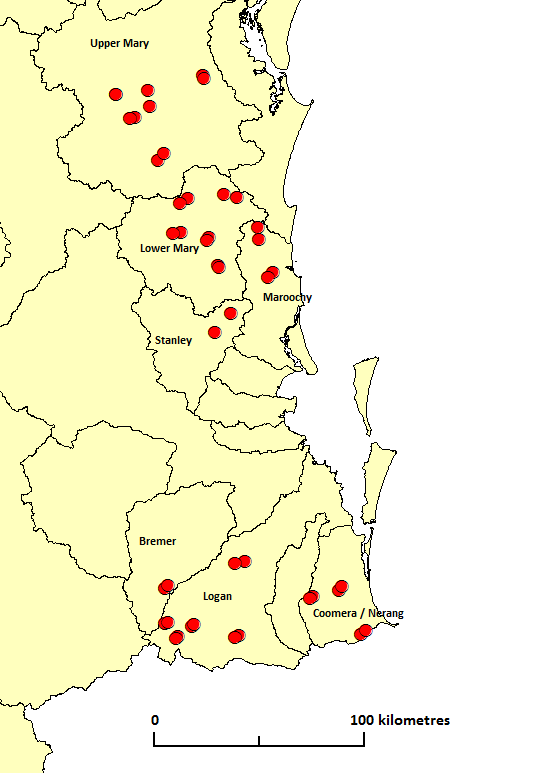
\includegraphics[width=12cm,keepaspectratio=true]{map.png} % figures can be in pdf, png, jpeg or eps format
\caption[Map of study areas described in Chapters 2 and 3.]{\small{Map showing study areas, and geographical distribution of field sites described in Chapters 2 \& 3 (lower left) and 4 (lower right) (Google Maps 2015).}\label{fig:Ch6_F1}}
%\label{Ch6_F1} % label for cross-referencing
\end{center}
\end{figure}   
\clearpage

\section{Ecological responses of riparian plant communities to fluvial hydrology}
The relationship between environmental heterogeneity and biodiversity has been a key focus of ecologists since the early 1960’s \citep{MacArthur1961, Stein2014}. Riparian landscapes provide particularly useful model systems for exploring hypotheses about environmental heterogeneity due to strong control of biotic assemblages by fluvial hydrology. In tandem with disturbance, hydrologically-driven environmental heterogeneity has taken a central role in our conceptualisation of how riparian ecosystems function \citep{Poff1997, Naiman2005}.

Chapters 2, 3 and 4 tested hypotheses derived from this paradigm. Broadly, this work confirms the importance of hydrological heterogeneity and fluvial disturbance in shaping riparian plant assemblages. The specific contribution of these chapters to the riparian literature lies in the mechanistic, functional trait-based approach used. Through the lens of functional traits, I have begun to address questions about how flow regime influences ecological strategies of riparian plants at the community level, and how the functional organisation of communities varies along hydrological gradients.

In Chapter 2, I found that wood density, a functional trait associated with resistance to mechanical disturbance and drought tolerance \citep{Chave2009, Niklas2010}, varied strongly in response to patterns of hydrology. Community mean values of wood density increased with the intensity of fluvial disturbance and flow heterogeneity; communities which experienced more variable flow conditions were shifted towards the ‘slow’, conservative end of the spectrum of resource-economic ecological strategies \citep{Reich2014a}. Wood density in turn influences wood decomposition rates \citep{Mori2013} which has implications for ecosystem nutrient cycling and energetic fluxes in riparian ecosystems \citep{Harmon1986}, as well as for the residence time of geomorphically active large woody debris in river systems {\citep{Gurnell2002, Cadol2010}. I also found a humped relationship between community-weighted variance in wood density and the same combined gradient of disturbance and hydrological heterogeneity, lending evidence to general hypotheses (from outside of the riparian literature) that intermediate levels of disturbance should promote divergence in disturbance-response strategies \citep{Grime2006, Sonnier2010}. Given the substantial cost to plants incurred in setting down dense woody tissue \citep{Falster2006}, these findings demonstrate that some of the key trade-offs negotiated by plants in riparian communities are made in response to fluvial disturbance and hydrological heterogeneity.
 
Plant life forms and qualitatively derived functional groups have been used for some time to describe functional organisation in riparian plant communities \citep{Brinson1993, Stromberg2010, Stromberg2013}. In Chapters 3 \& 4 I derived quantitative, continuous indices of functional diversity from vegetation survey and data for a range of functional traits with the intent of capturing key axes of variation in riparian plant ecological strategy. Using functional traits as descriptors of ecological strategy provides generality across systems \citep{Lavorel2002, Suding2008}, and negates any requirement for expert knowledge to assign species to qualitative functional groups. These indices of functional diversity also facilitate the use of quantitative modelling methods \citep{Mason2013}, and allow more solid inferences to be made about how individual components of flow regime influence community assembly and ecosystem processes than are possible using taxonomic metrics of diversity \citep{Tilman1997, Diaz1998}.

Patterns of variation in functional dispersion measured in natural landscapes of coastal south-eastern Australia (described in Chapter 3) showed strong positive relationships with metrics describing hydrological heterogeneity. While I did not systematically describe variation in species richness along hydrological gradients, species richness (but not the number of species used in the functional dispersion analysis) was significantly positively correlated with functional dispersion. I was able to generate a multiple regression model which explained 80 \% of the total variation in functional dispersion using three hydrological metrics. Partitioning of variance between this model and optimal models generated using climatic and soil variables, showed that a substantial proportion of variance explained by hydrology was not co-explained by climate or soil, further demonstrating the dominance of fluvial disturbance and flow variability in shaping the functional structure of these plant communities.

Riparian plant communities in south-eastern Queensland (described in Chapter 4) showed somewhat different responses to hydrology. Several additional environmental variables were taken into account to quantify the degree of anthropogenic modification both to the surrounding catchment and to the flow regime itself. In this study, I found functional richness and functional divergence (as measured by abundance-standardised functional dispersion) were associated with only a limited subset of metrics describing hydrological heterogeneity, and variance partitioning of models showed that relatively little variation in either functional richness or divergence was explained by hydrology when climate and soil properties were taken into account. Flow modification did explain some variation in metrics of functional diversity, but again, not independently. Contrary to our hypotheses, and to patterns commonly described in Northern hydroecological systems ({e.g. \citep{Naiman1997}), species richness declined as flow regimes became more heterogeneous. The observation that species richness and metrics of functional diversity showed opposite relationships with the same hydrological variables allowed us to determine that communities living under hydrologically heterogeneous conditions were maintaining functional diversity with a reduced species pool. 

\subsection{Outstanding questions about the role of hydrological heterogeneity in structuring communities}
Although hydrology was the dominant control on functional traits and functional trait diversity in both regions analysed here, the relative importance of hydrological heterogeneity per se differed. Some of the major outstanding questions in this thesis are why this might have been so, and which aspects of the findings can be generalised or extrapolated to systems in other regions within Australia and across the globe?

It is possible that Australian plant communities in fact have unique relationships with flow heterogeneity, given Australia's title of 'the planet’s most hydrologically variable continent' \citep{Peel2004, Rustomji2009}. A larger comparative study of factors shaping the functional ecology of riparian plant communities would be an essential step towards finding generalities in flow heterogeneity-diversity relationships, and would also provide further opportunity to investigate discontinuities in trends. Riparian researchers are becoming more interested in functional ecology, and it is possible that we will see global syntheses being made over the next decade. Research in regions underrepresented in the riparian ecology literature, such as the tropics and the developing world, would be of particular value in this endeavour.

Absent an exhaustive global comparative synthesis, comparing the specific findings of Chapter 3 and Chapter 4 reveals a possible explanation for their differences. While functional diversity of communities described in Chapter 2 scaled monotonically with most metrics of flow variability, and was positively associated with species richness, functional diversity of communities in south-east Queensland (Chapter 4) was significantly associated with only a small set of metrics describing flow variability (e.g. interannual variability in baseflow index, constancy of monthly maximum flows) and in those cases, relationships were better described by quadratic models. As noted previously, species richness showed inverted relationships with these metrics. To properly compare the results of these two chapters, a methodological issue must first be addressed: functional dispersion (FDis), \textit{sensu} Laliberté and Legendre \citep{Laliberte2010}, was used in Chapter 3, while standardised effect size FDis (FDis.SES), \textit{sensu} \citep{Mason2013}, was used in Chapter 4 as a measure of functional divergence. With the exception of a few outliers, FDis was tightly positively correlated with FDis.SES for the south-east Queensland dataset (Pearson's r = 0.75). With respect to species richness, this confirms that standardising FDis for abundance was not responsible for inverting the species richness – functional diversity relationship.

In our discussion of Chapter 4, I noted that rhythmicity in temporal patterns of energy and resource availability and environmental heterogeneity may both act as controls on riparian plant diversity. I citepd recent work showing that rhythmic seasonal flow activity fosters greater diversity in birds and fishes and greater net primary production in plant communities \citep{Jardine2015}, and that energy (and resource) availability may be more important than environmental heterogeneity in determining patterns of diversity \citep{Lundholm2009}. Thus differences between the findings of Chapters 3 and 4 could be explained by differences in the influence of these two factors. For this conceptual model to be useful, we need to describe some key components of its structure. Firstly, is it flow rhythmicity \textit{per se} which is important, or simply total energy availability, which happens to be maximised in rhythmic systems? If the former, can flows be both heterogeneous and rhythmic, or are the two factors inherently opposite? For example, can a river with high interannual variability in its baseflow index also experience highly regular summer flood flows? Perhaps cases at extreme ends of each spectrum are less interesting than those at intermediate levels of heterogeneity and energy availability / rhythmicity.
 
Perhaps a better way of conceptualising environmental control over diversity might be as a three dimensional relationship, where heterogeneity and energy availability (or flow rhythmicity) are incompletely orthogonal to each other. The curves presented in this thesis would then be two dimensional slices of a three dimensional volume. A challenge for future research in this field is therefore to explicitly include energy availability or flow rhythmicity in hypotheses about flow responses of plant communities, and to attempt to characterise how communities respond to both factors simultaneously.

\section{Responses of riparian plant communities to anthropogenic environmental change}
My interest in the functional ecology of riparian plant communities was initially motivated by the need for new approaches and perspectives towards conserving, rehabilitating and managing riparian landscapes in south-eastern Australia. The 20th century has seen unprecedented change in riverine ecosystems and these changes are likely to intensify over the current century \citep{Nilsson2000, Hennessy2008}. Compared with Europe and North America, applied river rehabilitation in Australia is somewhat hampered by a lack of basic ecological knowledge \citep{Brooks2007}. Thus one of the main aims of this thesis was to inform management with new information about riparian ecology in both natural and modified landscapes.

\subsection{How might riparian plant communities respond to climate change?}
Climate change is predicted to have global impacts on ecosystems in the 21st century \citep{IPCC2014}. Riparian ecosystems are likely to be particularly vulnerable due to their high exposure and sensitivity to changes in climate, in combination with pressures associated with extraction of provisioning ecosystem services by humans \citep{Capon2013}. Elevated concentrations of carbon dioxide (eCO\textsubscript{2}) represent the most direct and obvious change to the atmosphere. The potential influence of eCO\textsubscript{2} on plants and plant communities has been the topic of intensive research over the last two decades. To date, however, the implications for conservation management under high CO\textsubscript{2} regime are highly species and system specific, and are likely to be contingent on a slew of other environmental factors \citep{Poorter2003a, Norby2011, Poorter2011, Reich2014}. Basic research on the ecological effects of eCO\textsubscript{2} is needed for individual systems, and each piece of experimental work contributes to the greater outlook.

Of the three anthropogenic alterations investigated in this thesis, I suggest that elevated atmospheric CO\textsubscript{2} (eCO\textsubscript{2}) may have the smallest effect. I showed in Chapter 5 that eCO\textsubscript{2} significantly stimulated growth in only one of three riparian tree seedlings, and this effect was completely negated by inundation. Inundation itself had strong effects on gas exchange, growth and functional traits in all three species. Differential responses between species to combined waterlogging and eCO\textsubscript{2} may have flow-on effects to demographics, competition, and ultimately, community composition.
 
Chapter 5 contributes to what is currently a very small set of publications investigating the potential for interactive effects between future atmospheric concentrations of CO\textsubscript{2} and inundation or waterlogging events on terrestrial plants \citep{Megonigal2005, Shimono2012, Arenque2014}. I included an analysis of functional trait responses, as well as including a recovery phase in the experiment, neither of which have been previously attempted to our knowledge. Fruitful avenues for future work include study of more species, serial waterlogging treatments to better understand how eCO\textsubscript{2} influences on waterlogging recovery, analysis of leaf nutrient concentrations to determine the role of nutrient limitation in suppressing growth stimulation by eCO\textsubscript{2} \citep{Reich2014}, and mesocosm experiments to investigate the implications of eCO\textsubscript{2} – waterlogging interactions for competition.

Greater hydrological variability and intensity of extreme weather events characterise models of high CO\textsubscript{2} climates \citep{Hennessy2008, stocker2013climate}. Our research demonstrates that riparian plant communities vary substantially in their taxonomic and functional composition over gradients of hydrological heterogeneity. As discussed in Chapters 2 and 3 \citep{Lawson2015, Lawson2015a}, the changing climate is likely to enhance dominance of variability-tolerant ecological strategies associated with traits such as high wood density, and push communities towards more dispersed functional structures. In species-rich communities of south-east Queensland, increased flow heterogeneity may have important consequences for taxonomic diversity, functional redundancy and ecosystem resilience. Greater exotic abundance was associated with more heterogeneous systems in south-eastern Queensland. Despite the lack of association between flow modification and exotic abundance in this study, it remains possible that climate-related increases in hydrological heterogeneity may also result in invasion by exotic species.

Further work is required to integrate observations about riparian plant community responses to hydrological heterogeneity with climate change predictions. Functional trait approaches are likely to be particularly useful in the absence of detailed species-level ecological knowledge \citep{Catford2012a}.

\subsection{Could environmental flows be a useful tool for river rehabilitation in south-eastern Australia?}
Hydrology was confirmed as the ‘master variable’ controlling riparian plant communities \citep{Poff1997} in both field studies, but flow modification also had a profound influence on species richness in south-eastern Queensland. That homogenised flows were actually associated with increased species richness (and functional diversity, to some extent) runs counter to much of the riparian literature on flow modification \citep{Nilsson2000, Lytle2004}. As discussed above, increased flow rhythmicity may underlie this unexpected effect. The lack of any association between flow modification and abundance of exotic species also opposes the general body of literature \citep{Catford2011, Greet2012}. Catchment land use and soil properties explained a substantial proportion of variation in exotic abundance, and may be more important drivers of invasion in this region.

Environmental flows - flows released from dams which are engineered to mimic natural flow events - are the focus of increasing research effort, and may be an important tool in rehabilitation of modified systems \citep{Arthington2012}. Frameworks for developing and using environmental flows, such as Ecological Limits of Hydrological Alteration (ELoHA) \citep{Poff2010a}, are predicated on the notion that altered flow regimes are the main cause of degradation in riparian ecosystems. The relationship between flow alteration and degradation is clearly defined in some systems, such as those invaded by Tamarix spp. in south-western North America: flood reduction and homogenised flow regimes result in more invasive \textit{Tamarix spp.} and less native \textit{Populus spp.} \citep{Stromberg2007, Shafroth2010}. Our analysis of patterns of functional diversity in natural landscapes (Chapter 3) led us to conclude that managers should include a component of variability in designed flow regimes to simulate natural flow heterogeneity. In south-east Queensland, the situation is more complicated, and the feasibility of using environmental flows for conservation or restoration depends on the desired outcome. Supporting indigenous biodiversity over exotic species, improving geomorphic condition, generating habitat complexity and maintaining or restoring lost ecosystem processes and services are commonly desired outcomes for environmental flows \citep{Richter2007, Poff2010a, Meitzen2013}. South-east Queensland communities were particularly sensitive to modification of contingency of monthly minimum flows (year on year variability in monthly minimum flow patterns), suggesting management efforts aimed solely at maximising taxonomic diversity would do well to increase flow contingency. This approach risks shifting community composition, but may be a reasonable response to offset greater climatic variability under future climates. Our research in south-east Queensland had rather less to say about the potential utility of environmental flows in directing functional diversity and associated ecosystem functionality. Flow modification largely did not have a consistent effect on functional diversity, suggesting that funds and effort may be better spent on local initiatives within catchments, such as improving landholder engagement in rehabilitation projects \citep{McDonald2009}.

\section{Conclusion}
Awareness of the economic, societal and intrinsic value of Australian waterways is increasing, and the field of riparian ecology is now progressing rapidly in Australia. We are finding commonalities with more extensively studied river systems in other parts of the world, and also new patterns and processes which give Australian river systems a unique character.  I attempted to answer some basic questions about riparian plant communities in south-eastern Australia using methods from modern plant ecology. In my first two studies I was able to clearly validate my hypotheses, while in the third and fourth studies a more complex and unexpected picture arose. Hopefully, I have set a useful stage for further work on the functional ecology of riparian plant communities, and my basic research informs more applied aspects of river management and rehabilitation.

%%%%% REFERENCES % this is in a new chapter due to the memoir format
\renewcommand\bibname{{References}} 
\begin{small}
\bibliographystyle{apalike}
\bibliography{library}
\end{small}


\end{document}

